\documentclass[titlepage,a4paper,10pt]{article}
% Språk och encodings
\usepackage[swedish,english]{babel}
\usepackage[T1]{fontenc}
\usepackage[utf8]{inputenc}
\usepackage[fixlanguage]{babelbib}
% Images and floats
\usepackage{graphicx}
\usepackage{wrapfig}
\usepackage{float}
% Clear type + Sans-serif font
\usepackage{lmodern}
\renewcommand{\familydefault}{\sfdefault}
% Matte
\usepackage{amsmath, amsthm, amssymb}
% Algoritmer
\usepackage[ruled,vlined]{algorithm2e}
% Länkar
\usepackage{color}
\definecolor{dark-blue}{rgb}{0, 0, 0.6}
\usepackage{hyperref}
\hypersetup{
  colorlinks=true,
  linkcolor=dark-blue,
  urlcolor=dark-blue
}
% Vettiga paragrafer
\setlength{\parindent}{0pt}
\setlength{\parskip}{2ex}

% Sidhuvud/sidfot
\usepackage{fancyhdr}
\setlength{\headheight}{15pt}
\pagestyle{fancyplain}
\lfoot{Carl-Oscar Erneholm \\ 880422-0872 \\ coer@kth.se}
\rfoot{Martin Nycander \\ 881028-0076 \\ mnyc@kth.se}
\cfoot{Page \thepage}

% Språk
\selectbiblanguage{swedish}
\selectlanguage{swedish}

% Titel
\title{ID1217: Parallel Particle Simulation}
\author{Martin Nycander \and Carl-Oscar Erneholm}
\date{\today}

\begin{document}
\maketitle

\tableofcontents
\newpage

\setcounter{page}{1}
% In your report you should explain what you have done and what you have learned.
% Your report should be few (about 10) pages of text plus tables and figures and an optional Appendix.

\section{Problem definition}

%TODO: An Introduction to the problem.
    \subsection{Parallelized Particle Simulation}

    The task was to optimize and parallelize a particle simulator, we
    where given four implementations of the simulator: one running sequentially,
    one parallelized using pthreads, one parallelized using openmp and one
    parallelized using MPI. The given simulator implementation made $n^2$
    computations each frame, where $n$ is the number of particles.

    But in contrast to the traditional N-body problem this simulation only
    simulates the interaction between particles within a certain distance from
    each other, moreover the density of particles are set low enough so that
    only $O(n)$ interactions are expected at any given moment. Therefore it
    should be possible to do the necessary calculations for each frame in
    $O(n)$, this is the first task. Once all implementation runs the
    computations in $O(n)$ %TODO: ... Time to optimize the parallel implementations.

    % Not needed?
    %\subsection{Not quite N-body problem} %TODO: Dig in deeper on the math, lead into the solution explained in the next section. How we can make this O(n).


\section{Problem solutions}

%TODO: describe how we made the serial program O(n), talk about grids.
    \subsection{Simulation Design}

        Each frame the original implementation made $n^2$ computations, for each
        particle it calculated the distance of each other particle, it the
        particle was close enough it also calculated the real effect, and
        applied the appropriate force to the particle. 

        \begin{equation}
            gridSize = \frac{\sqrt{0.0005 \cdot n}}{0.01} + 1 \\
        \end{equation}
        \begin{equation}
            grid.size = gridSize^2 = \left(\frac{\sqrt{0.0005 \cdot n}}{0.01} + 1\right)^2
        \end{equation}

    \subsection{Parallelization Design with Shared Memory}% TODO: A description of the synchronization you used in the shared memory implementation.

    \subsection{Parallelization Design with Distributed Memory}% TODO: A description of the communication you used in the distributed memory implementation.

    %Maybe this does not need its own seciton? TODO
    \subsection{Design Decisions}% TODO: A description of the design choices that you tried and how did they affect the performance.

\section{Results}

% TODO: A plot in log-log scale that shows that your serial and parallel codes run in O(n) time and a description of the data structures that you used to achieve it. In order to get more precise timing estimates, we recommend you to run a program at least 5 times and take the median (rather than the mean) of the simulation times.

% TODO: Speedup plots that show how closely your parallel codes approach the idealized p-times speedup and a discussion on whether it is possible to do better.
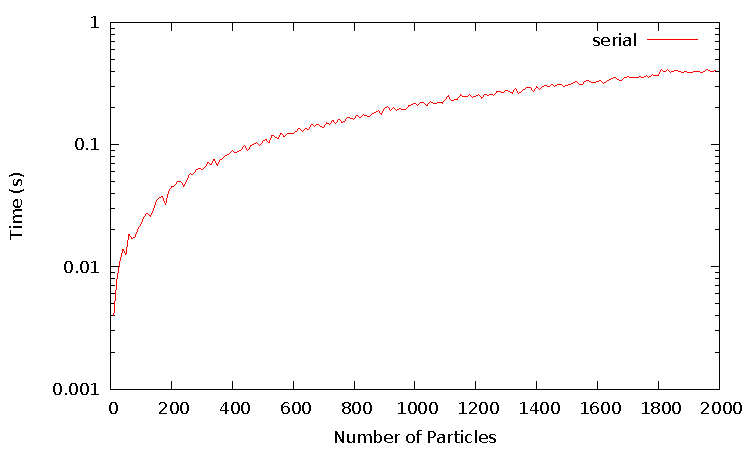
\includegraphics{plots/serial.pdf}
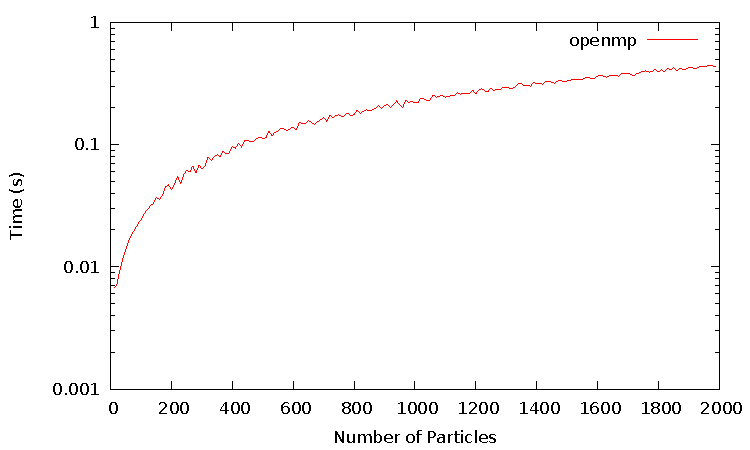
\includegraphics{plots/openmp.pdf}
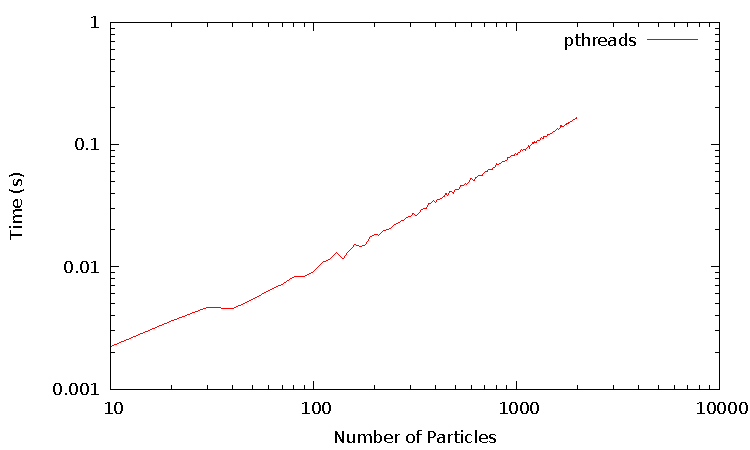
\includegraphics{plots/pthreads.pdf}
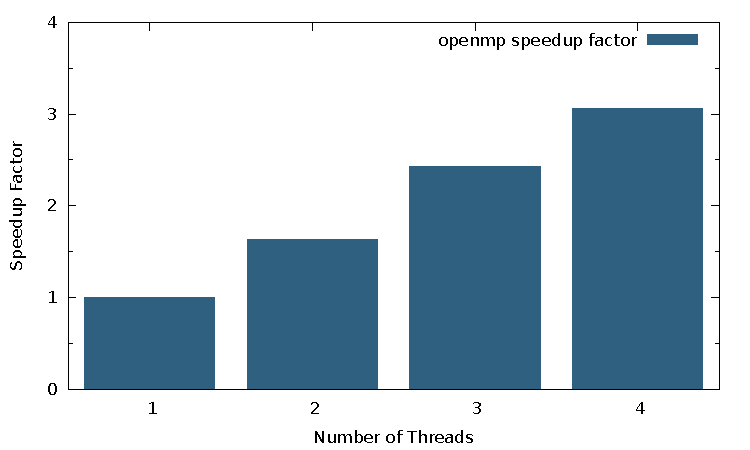
\includegraphics{plots/openmp_speedup.pdf}
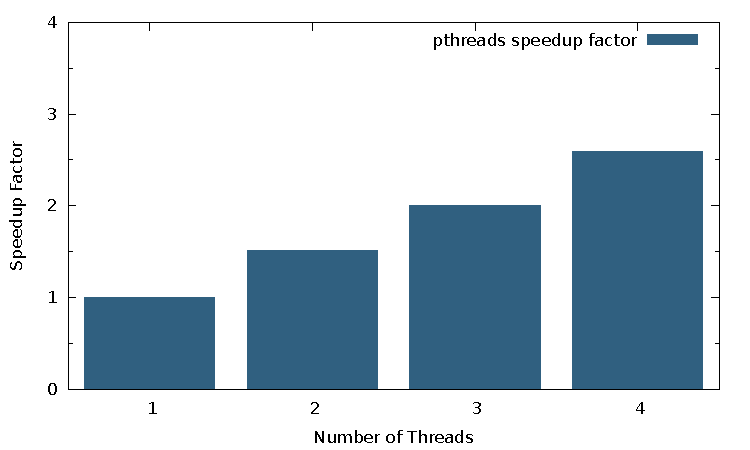
\includegraphics{plots/pthreads_speedup.pdf}

% TODO: Where does the time go? Consider breaking down the runtime into computation time, synchronization time and/or communication time. How do they scale with p?

\section{Discussion}

% TODO: A discussion on using pthreads, OpenMP and MPI.

\end{document}
